\section{Implementation: \textnormal{\textit{available framework overview and main components}}}
\begin{figure}[t]
	\centering
	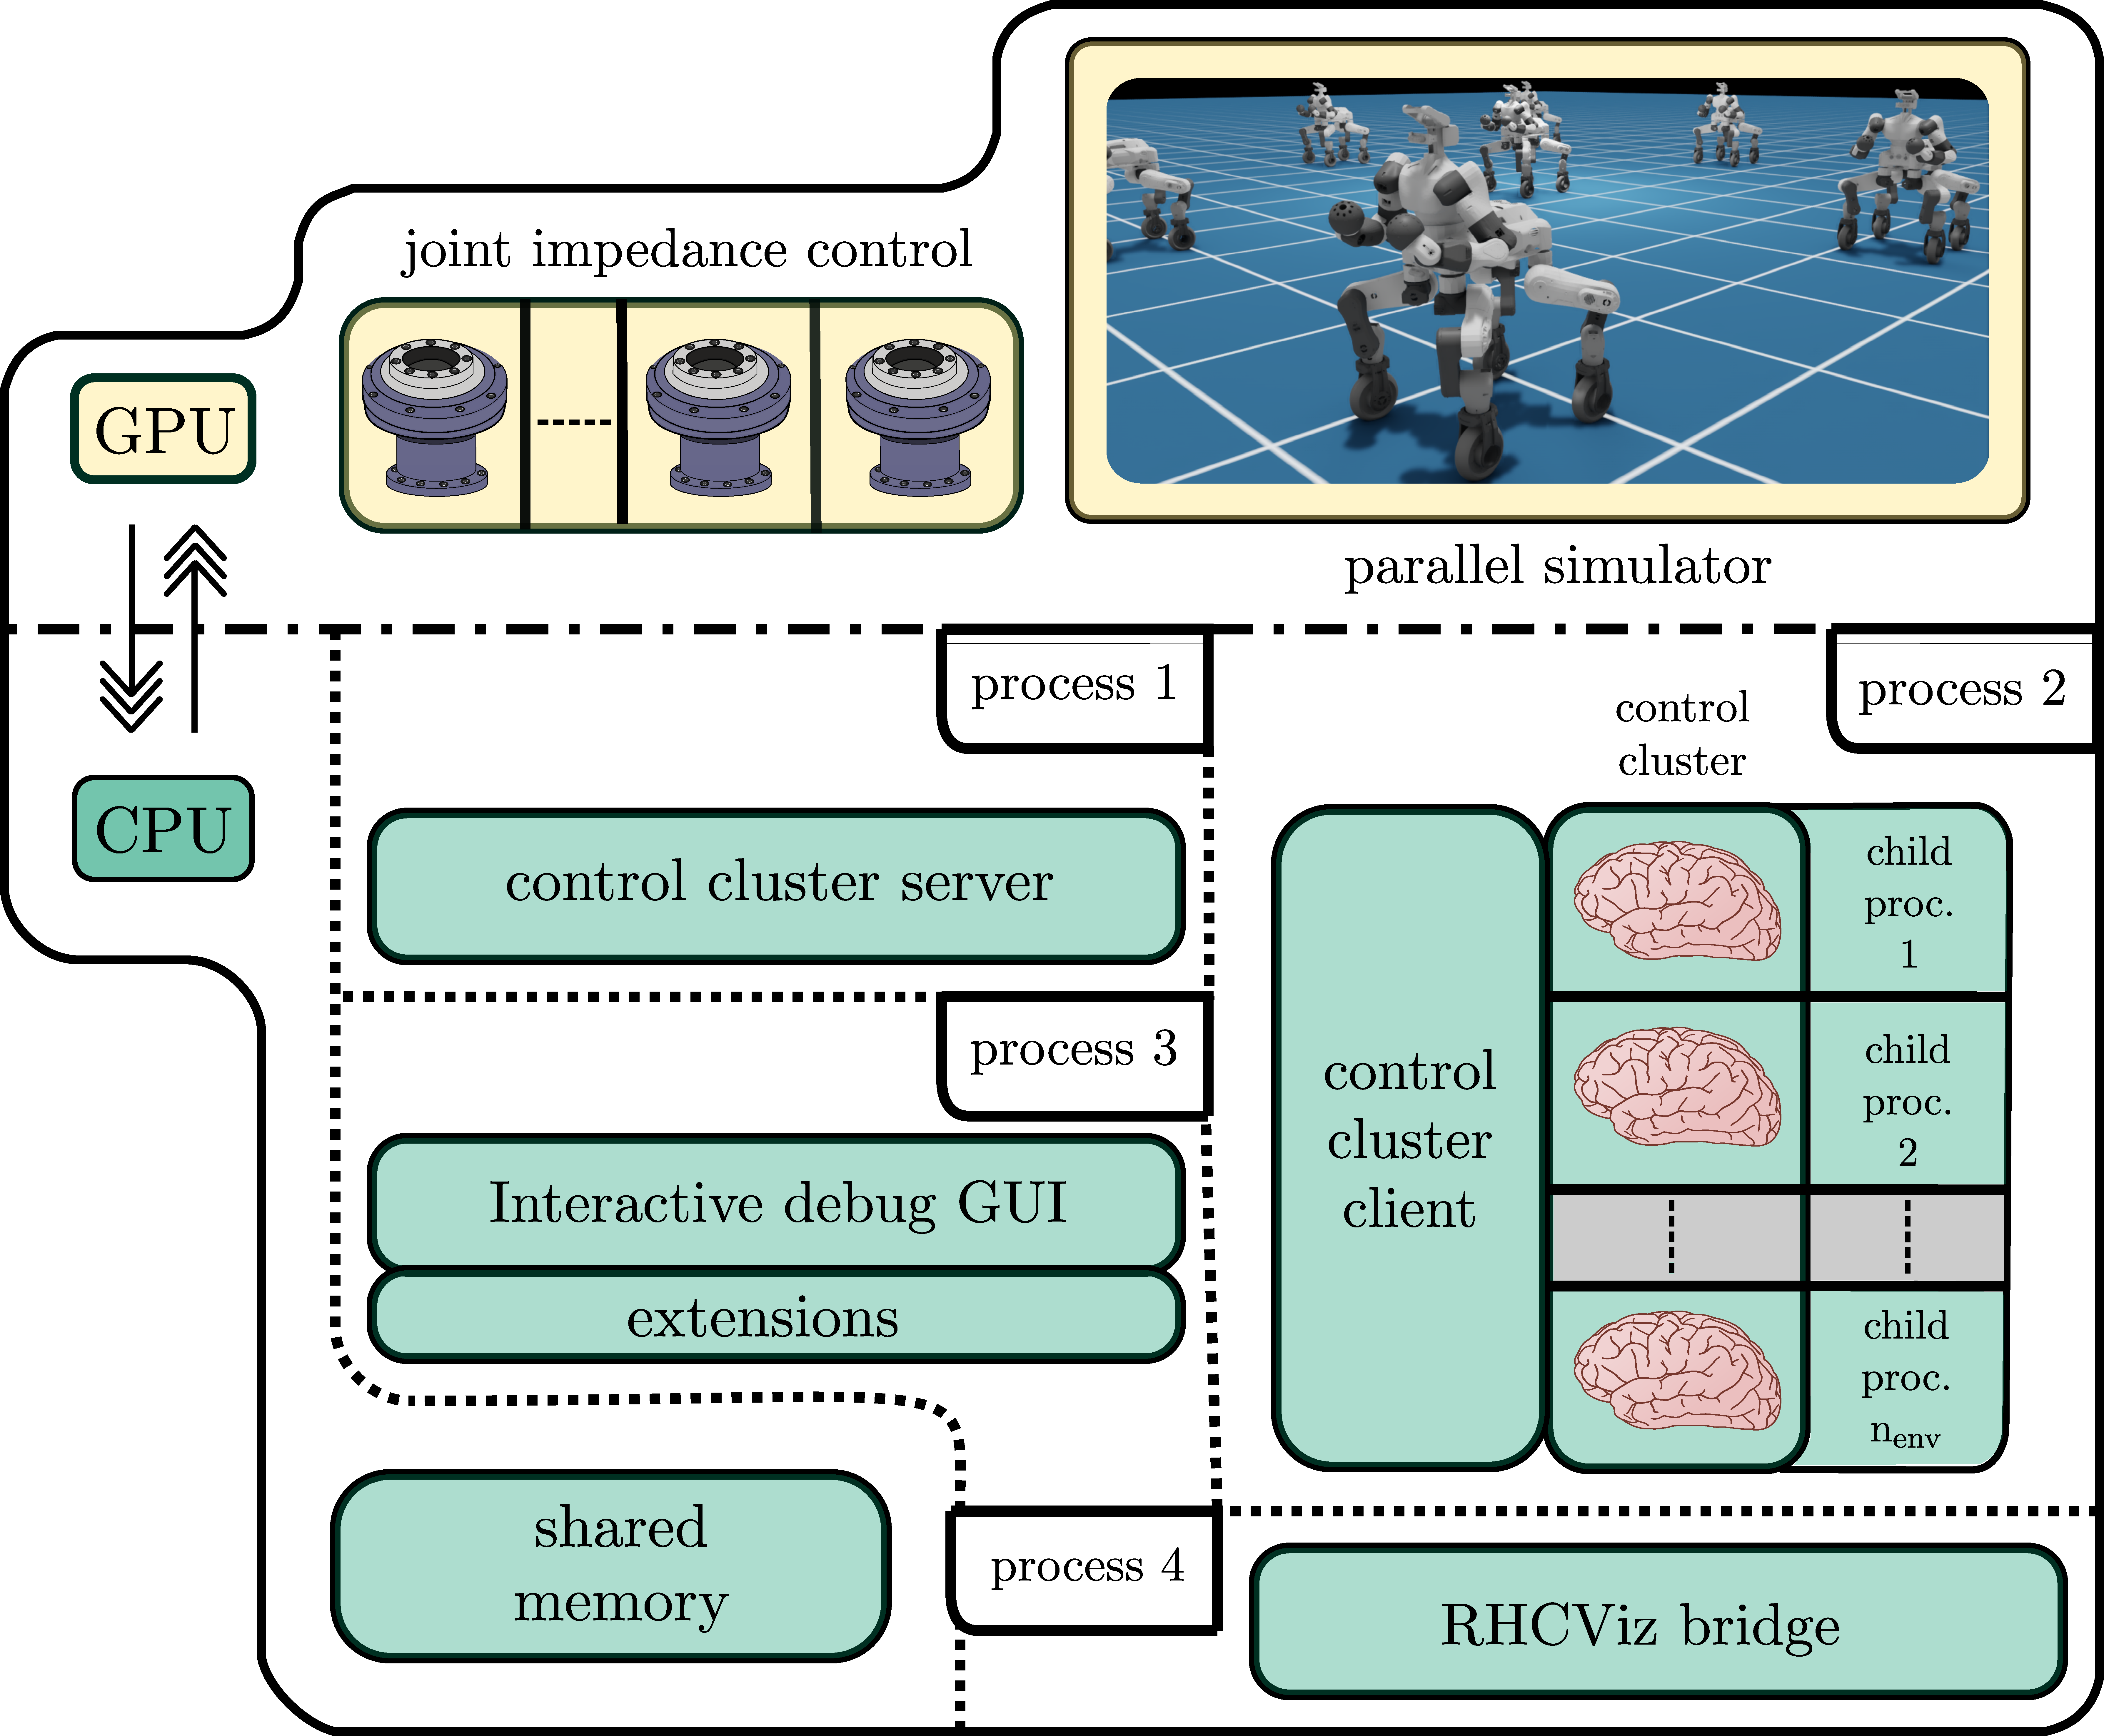
\includegraphics[width=0.9\columnwidth]{imgs/cocluster_arch.pdf}
	\caption{High-level overview of the software implementation of the training environment to which the agent is exposed: the robot in the simulator is controlled through a joint-level impedance controller, which is in turn used by a higher-level receding horizon controller. The agent can indirectly control the robot through the latter. The training environment lives in an independent process and uses shared memory for interacting with the simulation environment.}
	\label{fig:coclbridge_arch}
\end{figure}
The advent of accurate GPU-accelerated simulation tools~\cite{web::isaacsim,rl:mujocoaccelereted2023} allows for a massive decrease in the training wall-time for data-hungry algorithms like RL and facilitates real-world deployment through domain randomization~\cite{rl:rudin2022learning,rl:rudin2022advanced}. We consequently choose \textit{Omniverse IsaacSim}~\cite{web::isaacsim} as the simulation backend, while we use PyTorch for all deep-learning related components and  \textit{Horizon}~\cite{frameworks::horizon_to} for formulating and running RHC controllers (on CPU, with an iLQR solver backend). One big drawback of this approach is the presence of the controllers on CPU, which currently represents our bottleneck in terms of training performance and parallelization capacity.
Fig.~\ref{fig:coclbridge_arch} shows a high level software overview of the main moduli the echosystem is made of. Specifically, we developed the following software modules:
\begin{itemize}
	\item \textit{SharsorIPCpp}~\cite{mystuff::sharsoripcpp} serves as the shared memory backend for fast data sharing and synchronization between all components on CPU.
	\item \textit{OmniRoboGym}~\cite{mystuff::omnirobogym} is used as a wrapper around IsaacSim and provides an interface to the \textit{simulation} environment.
	\item \textit{CoClusterBridge}~\cite{mystuff::coclusterbridge} exploits~\cite{mystuff::sharsoripcpp} and coordinates the connection and synchronization between the simulation environment and a cluster of RHC controllers. It furthermore provides abstractions for the controllers and an extensible debug GUI for monitoring the cluster.
	\item \textit{RHCViz}~\cite{mystuff::rhcviz} is a debug tool based on ROS1/ROS2 and RViz for visualizing RHC solutions in real-time. For our specific use case, it also allows to inspect a single environment during training without the need of any rendering on the simulator side.
	\item \textit{LRHControl}~\cite{mystuff::lrhccontrol} is the main package of the echosystem and is responsible for setting up and running the simulation environment, the control cluster and the training environment.
\end{itemize}




